\documentclass[conference]{IEEEtran}
\IEEEoverridecommandlockouts
% The preceding line is only needed to identify funding in the first footnote. If that is unneeded, please comment it out.
\usepackage{cite}
\usepackage{amsmath,amssymb,amsfonts}
\usepackage{algorithmic}
\usepackage{graphicx}
\usepackage{textcomp}
\usepackage{xcolor}
\usepackage{mdframed}
\definecolor{shadecolor}{rgb}{0.21,0.21,0.21}
\def\BibTeX{{\rm B\kern-.05em{\sc i\kern-.025em b}\kern-.08em
    T\kern-.1667em\lower.7ex\hbox{E}\kern-.125emX}}
\begin{document}

\title{Different Classification Schemes for Medical,Railway Booking and Fashion Data\\}

\author{\IEEEauthorblockN{Parth Shah}
\IEEEauthorblockA{\textit{Computer Science and Engineering} \\
\textit{Indian Institute of Technology,Delhi}\\
New Delhi, India \\
email address}
\and
\IEEEauthorblockN{Aditya Jain}
\IEEEauthorblockA{\textit{Computer Science and Engineering} \\
\textit{Indian Institute of Technology,Delhi}\\
New Delhi, India \\
email address}
\and
\IEEEauthorblockN{Piyush Mittal}
\IEEEauthorblockA{\textit{Electrical Engineering} \\
\textit{Indian Institute of Technology,Delhi}\\
New Delhi, India \\
email address}
}

\maketitle

\begin{abstract}
Have to write the Abstract in the end summarizing all the work
\end{abstract}

\begin{IEEEkeywords}
component, formatting, style, styling, insert
\end{IEEEkeywords}

\section{Introduction}
This is a report made by observing results of various supervised and unsupervised classification techniques over a set of three databases for various different parameters. Python was used to implement all the classifiers and in taking their results. Bayes Classifier , Naive Bayes Classifier were the supervised classification techniques while for unsupervised K-Means and K-Nearest Neighbour Classifier were used. The three datasets were of a Medical Training , Railway Booking and Fashion Mnist. Principal Component Analysis (PCA) was used in the case of Fashion Mnist for dimension reduction of its large dimension. In this paper we will seek the answer of the following questions:
\begin{mdframed}
    1) Which Classifier gives best accuracy for different Data Sets?\newline
    2) What are the impacts of changing the parameters of the classifiers?
\end{mdframed}
Now we will discuss each classifier separately and how the data was classified in each of them. But before going further let's take a look at the given data for its better understanding.
\section{A Look At The Given Data}
\begin{enumerate}
    \item \textbf{Medical Training:} It contains values of three medical tests conducted, all of which are continuous. Each set of the test values determine what is the status of the health (HEALTHY, SURGERY,MEDICATION).Because of the low dimensions of the feature vector we do not need to apply PCA in this data set.
    \item \textbf{Railway Booking:} It contains data of people who booked a ticket on some train. There are 7 parameters associated with every person. Of which some are categorical and others continuous. Because of this there are different methods for finding distances for KMeans and K-NN. Classification is to be done based on whether the person boarded or not.
    \item \textbf{Fashion Mnist:} It contains 10 classes of images each of dimension 784. With 70000 samples it is the largest data set given and applying PCA on it is a wise choice. Each value of the feature vector is continuous. 
\end{enumerate}

\section{Bayes Classifier}
\subsection{Medical Training Data}

\subsection{Train Data}

\subsection{Fashion MNIST}

\section{Naive Bayes}
\subsection{Medical Training Data}

\subsection{Train Data}

\subsection{Fashion MNIST}

\section{\textbf{K-Means Classifier}}
K-Means is one of the variants of the EM algorithm with the assumptions that clusters are spherical. It is a widely used clustering algorithm. Now let's consider the algorithm :
\begin{itemize}
    \item Assigning each point to the most likely cluster based on distance from the centroid
    \item Recomputing the centroid from the newly assigned points
\end{itemize} 
We will see the results of the K-Means with random initialization first and then how different initialization schemes can have a better result.
\subsection{Advantage Of Seeding : \textbf{K-Means++}}
Instead of initializing the centroids randomly from the data if we choose them wisely we can gain substantial increase in speed and accuracy. In K-Means++ we assign the first centroid randomly and after that we select all the remaining centroids from a distribution of data points proportional to their minimum distances from the already chosen centroids.
\subsection{Medical Training Data}
\begin{table}[htbp]
\begin{center}
\begin{tabular}{|c|c|}
\hline
\textbf{Algorithm}&\textbf{\% Error} \\
\hline
\textit{K-Means with random init.} & 48.9\%\\
\hline
\textit{Scikit-Learn K-Means}& 48.63\%\\
\hline
\textit{K-Means++}&48.9\%\\
\hline
\multicolumn{4}{l}{$^{\mathrm{a}}$Clustered over all 3000 samples}
\end{tabular}
\label{tab1}
\end{center}
\end{table}
K-Means does not provide any benefit in this case as the sample is quite small already. Also the convergence was attained in around maximum 42 iterations in both cases. Since there were only 3 dimension feature vector PCA was not required. Euclidean distance was used as the measure of distance.
\subsection{Railway Booking}

\subsection{Fashion MNIST}
Doing classification without PCA is not feasible in this case so we tried different values of m(the reduced dimension).
\begin{table}[htbp]
\begin{center}
\begin{tabular}{|c|c|c|c|}
\hline
\textbf{Algorithm}&\textbf{m for PCA}&\textbf{number of iterations}&\textbf{\% Error} \\
\hline
\textit{K-Means with random init.} &2&34&56.25\%\\
\hline
\textit{Scikit-Learn K-Means}&2&NA&55.79\%\\
\hline
\textit{K-Means++}&2&43&56.11\%\\
\hline
\textit{K-Means with random init.} &5&50&51.04\%\\
\hline
\textit{Scikit-Learn K-Means}&5&NA&47.41\%\\
\hline
\textit{K-Means++}&5&37&44.08\%\\
\hline
\textit{K-Means with random init.} &10&76&45.68\%\\
\hline
\textit{Scikit-Learn K-Means}&10&NA&44.00\%\\
\hline
\textit{K-Means++}&10&48&44.40\%\\
\hline
\textit{K-Means with random init.} &10&66&44.25\%\\
\hline
\textit{Scikit-Learn K-Means}&10&NA&44.17\%\\
\hline
\textit{K-Means++}&25&36&41.96\%\\
\hline
\multicolumn{4}{l}{$^{\mathrm{a}}$Clustered over all 10000 samples}
\end{tabular}
\label{tab1}
\end{center}
\end{table}
\newline
To calculate accuracy for 10 classes we mapped our cluster number to the original class number which occurred most frequently.\newline
The table shows that how by reducing m we lose some our accuracy. But the computing time for higher values of m is very large. Also we can see how K-Means++ performs better and is almost on par with the scikit learn's method and for m=25 even produces better results. Also the number of iterations required to reach convergence were lower for K-Means++. Note that euclidean distance was used as the distance measure due to the continuous nature of the features.
\section{\textbf{K-Nearest Neighbour Classifier}}
K-Nearest Neighbour is the second unsupervised algorithm that was implemented.In this algorithms distances between all points and the test instance is calculated and the most frequent occurring class in the k nearest neighbours is assigned to the test instance. The best choice of k depends upon the data. Larger k ignores noise in the data while smaller k makes less distinction between different classes.
\subsection{Medical Training Data}
\begin{figure}[htbp]
\centerline{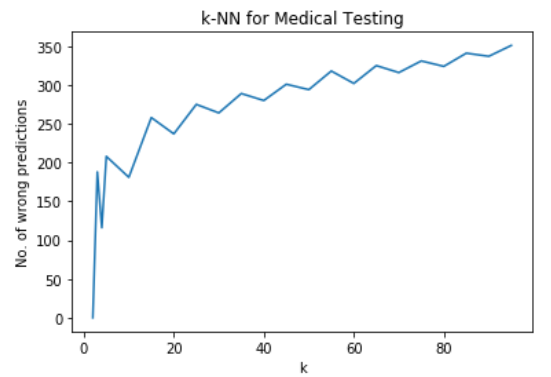
\includegraphics{knnmedical.PNG}}
% \caption{Example of a figure caption.}
\label{fig}
\end{figure}
So as the k increases the error is increasing because of less distinction between the boundaries of the different classes. Because of the continuous nature of the feature vector we used euclidean distance as the measure. The error \% of k-NN was very less than the one from k-Means e.g. for k = 3 error was 6.2\% only. 
\subsection{Train Data}
\begin{figure}[htbp]
\centerline{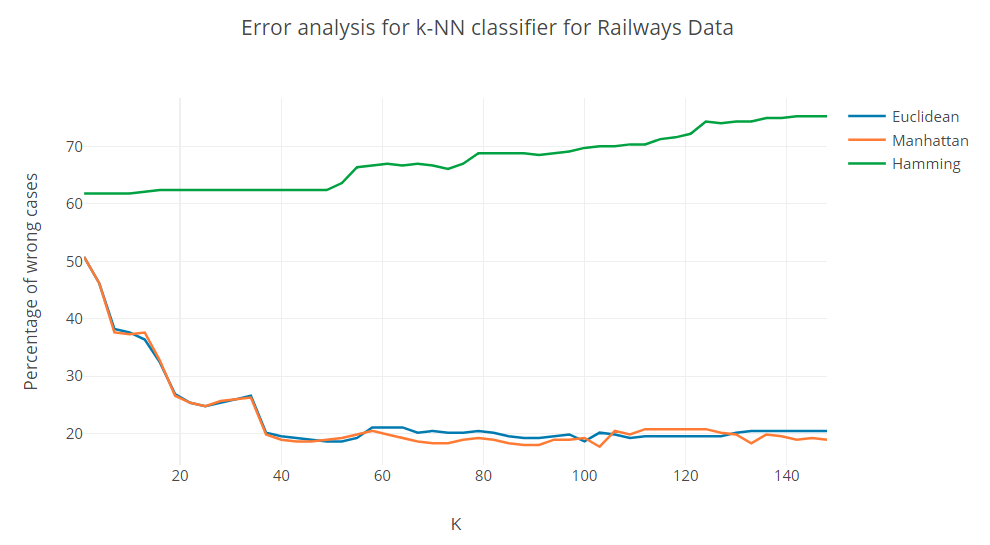
\includegraphics{knnrailways.PNG}}
% \caption{Example of a figure caption.}
\label{fig}
\end{figure}
With or without considering case ID parameter, the error lies in the range of 40-70 \% for normal and weighted classification under all type of distances but if we do normalization of data, we see a rapid decrease in error as k increases but not same for hamming distances and observe that error becomes stagnant after k=50.
\subsection{Fashion MNIST}
\begin{table}[htbp]
\begin{center}
\begin{tabular}{|c|c|c|}
\hline
\textbf{K}&\textbf{m (PCA)}&\textbf{\% Error} \\
\hline
\textit{1000} &2&45.31\%\\
\hline
\textit{1000}&5&64.2\%\\
\hline
\textit{6000}&5&66.4\%\\
\hline
\textit{100}&5&67\%\\
\hline
\textit{2}&5&64.2\%\\
\hline
\textit{500}&10&63.76\%\\
\hline
\multicolumn{4}{s}{$^{\mathrm{a}}$Neighbours from Training }
\end{tabular}
\label{tab1}
\end{center}
\end{table}

\section{Conclusion}

\section*{Acknowledgment}

The preferred spelling of the word ``acknowledgment'' in America is without 
an ``e'' after the ``g''. Avoid the stilted expression ``one of us (R. B. 
G.) thanks $\ldots$''. Instead, try ``R. B. G. thanks$\ldots$''. Put sponsor 
acknowledgments in the unnumbered footnote on the first page.

\section*{References}

Please number citations consecutively within brackets \cite{b1}. The 
sentence punctuation follows the bracket \cite{b2}. Refer simply to the reference 
number, as in \cite{b3}---do not use ``Ref. \cite{b3}'' or ``reference \cite{b3}'' except at 
the beginning of a sentence: ``Reference \cite{b3} was the first $\ldots$''

Number footnotes separately in superscripts. Place the actual footnote at 
the bottom of the column in which it was cited. Do not put footnotes in the 
abstract or reference list. Use letters for table footnotes.

Unless there are six authors or more give all authors' names; do not use 
``et al.''. Papers that have not been published, even if they have been 
submitted for publication, should be cited as ``unpublished'' \cite{b4}. Papers 
that have been accepted for publication should be cited as ``in press'' \cite{b5}. 
Capitalize only the first word in a paper title, except for proper nouns and 
element symbols.

For papers published in translation journals, please give the English 
citation first, followed by the original foreign-language citation \cite{b6}.

\begin{thebibliography}{00}
\bibitem{b1} G. Eason, B. Noble, and I. N. Sneddon, ``On certain integrals of Lipschitz-Hankel type involving products of Bessel functions,'' Phil. Trans. Roy. Soc. London, vol. A247, pp. 529--551, April 1955.
\bibitem{b2} J. Clerk Maxwell, A Treatise on Electricity and Magnetism, 3rd ed., vol. 2. Oxford: Clarendon, 1892, pp.68--73.
\bibitem{b3} I. S. Jacobs and C. P. Bean, ``Fine particles, thin films and exchange anisotropy,'' in Magnetism, vol. III, G. T. Rado and H. Suhl, Eds. New York: Academic, 1963, pp. 271--350.
\bibitem{b4} K. Elissa, ``Title of paper if known,'' unpublished.
\bibitem{b5} R. Nicole, ``Title of paper with only first word capitalized,'' J. Name Stand. Abbrev., in press.
\bibitem{b6} Y. Yorozu, M. Hirano, K. Oka, and Y. Tagawa, ``Electron spectroscopy studies on magneto-optical media and plastic substrate interface,'' IEEE Transl. J. Magn. Japan, vol. 2, pp. 740--741, August 1987 [Digests 9th Annual Conf. Magnetics Japan, p. 301, 1982].
\bibitem{b7} M. Young, The Technical Writer's Handbook. Mill Valley, CA: University Science, 1989.
\end{thebibliography}

\end{document}
